


\documentclass[11pt]{article} %Sets the default text size to 11pt and class to article.
%------------------------Dimensions--------------------------------------------
\topmargin=0.0in %length of margin at the top of the page (1 inch added by default)
\oddsidemargin=0.0in %length of margin on sides for odd pages
\evensidemargin=0in %length of margin on sides for even pages
\textwidth=6.5in %How wide you want your text to be
\marginparwidth=0.5in
\headheight=0pt %1in margins at top and bottom (1 inch is added to this value by default)
\headsep=0pt %Increase to increase white space in between headers and the top of the page
\textheight=9.0in %How tall the text body is allowed to be on each page

\usepackage{multicol}
\usepackage{graphicx}
\usepackage{vwcol}
\graphicspath{{./images/}}

\begin{document}
\centerline{\Large Manav Guglani}  %Makes whatever text you put in parenthesis move to the center
\noindent %Prevents the following text from being indented
\line(1,0){470}
\\  %This is the same as a return in Latex
 \parbox[t]{5cm}
{305, BH-7,\\
	NIT Uttarakhand\\
	Srinagar \\
	Garhwal-246174\\
	Uttarakhand}
%---------------------------%
\hspace{7cm}
\parbox[t]{3.5cm}
{Contact: 9548899230\\
	manav.ece14@nituk.ac.in\\
	\vspace{1pt}
	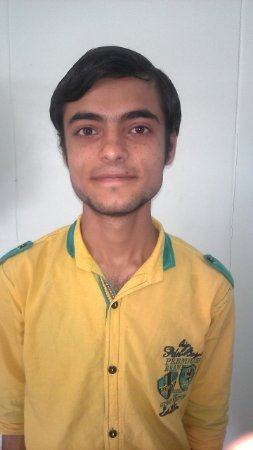
\includegraphics[scale=.2]{manav.jpg}
}
\section*{Objective}
\Large To excel in embedded systems and robotics and using this excellence to create useful products for growth of India. 
\section*{Education} 
\begin{tabular}{|c|c|c|c|c|}
	\hline
	Degree & College/School & University & Passing Year & cgpa or \% \\
	\hline
	B.tech & NIT Uttarakhand & NIT Uttarakhand & 2018 & 9.18\\
	\hline
	Intermediate & B.J.S. Public School & CBSE & 2013 & 90.40 \% \\
	\hline
	High School & B.J.S. Public School & CBSE & 2011 & 9.0 \\
	\hline
\end{tabular}
\section*{Projects}  
\begin{enumerate}
	\item Gas leakage detection robot
	\item Interfacing TSOP IR receiver with FPGA by Using Verilog HDL
	\item Wireless control of home appliances
	\item Self balancing robot
\end{enumerate}	
\end{document}
